
\section{Overview of Social Networking Platform Architectures}

Modern social networking platforms require high-throughput, low-latency architectures to handle the massive volumes of user-generated content and real-time interaction loops. Historically, social network designs relied on synchronous request-response patterns over traditional relational databases. However, research by Kwak et al. [1] demonstrates that the topology of modern social networks - characterized by low reciprocity, asymmetric follower-following relationships, and rapid information diffusion - fundamentally differs from classical human social networks, necessitating a shift toward event-driven architectures and distributed caching layers capable of handling real-time content propagation at scale.

A critical challenge arising from this scale of content production is information overload --- the cognitive burden imposed on users when incoming content volume exceeds their processing capacity. Gupta et al. [11] empirically demonstrated, across a large-scale sample study published in the Academy of Marketing Studies Journal, that unmanaged information streams are a statistically significant driver of emotional exhaustion and user fatigue on social media platforms. This finding is further substantiated by Stamenkovi{'c} and Aleksi{'c} [12], who applied the Stressor-Strain-Outcome (SSO) model to confirm that unfiltered digital overload leads to systematic information avoidance --- users disengaging from platforms entirely rather than engaging with irrelevant or overwhelming content. These findings collectively establish the academic necessity for intelligent content curation and ranking mechanisms within modern social networking systems.

\textbf{Comparison \& }\textbf{Breadit's}\textbf{ Positioning}

While legacy architectures utilize heavy database queries for feed generation, Breadit inherits the hybrid database model proposed by Carlson [2], combining PostgreSQL as the persistent relational source of truth with Redis as an in-memory database. Breadit differentiates itself by implementing this hybrid model within a TypeScript monorepo, using Prisma ORM to maintain strict type safety across database transactions while leveraging Redis to handle WebSocket adapter pub/sub states, minimizing backend connection overhead. Furthermore, directly addressing the information overload challenge identified by Gupta et al. [11] and Stamenkovi{'c} and Aleksi{'c} [12], Breadit incorporates a time-decay heuristic ranking algorithm on the Explore feed --- a design choice motivated by the empirical finding of Kwak et al. [1] that engagement signals (retweets, replies) are stronger predictors of content relevance than simple follower counts.

\section{Frontend Development Technologies}

\subsection{Overview of Frontend Frameworks}

Frontend technologies have transitioned from static HTML/CSS pages to highly dynamic, component-based frameworks such as React, Vue, and Angular. These modern frameworks enable reusability, state management, and efficient rendering, capabilities essential for micro-blogging platforms that require real-time updates, dynamic social feeds, and seamless navigation.

\subsection{Rationale for Choosing Next.js:}

Next.js is a powerful React framework widely adopted for building production-ready applications.

Key advantages include:
\begin{itemize}
  \item Server-Side Rendering (SSR) enhancing SEO and ensuring lightning-fast initial page loads for social feeds.
  \item Built-in Routing streamlining complex navigation across user profiles and communities.
  \item Seamless React Integration, leveraging component-based architecture and Virtual DOM for highly interactive user interfaces.
  \item Advanced optimization tools natively built-in for images, fonts, and external scripts.
\end{itemize}

For Breadit platform, where robust SEO, fast rendering, and real-time responsiveness are critical, Next.js provides the ultimate frontend foundation.

\section{Backend Development Technologies}

\subsection{Overview of Backend Languages}

Backend systems serve as the foundation for business logic, authentication, and database management. Common backend technologies include Java, Node.js, PHP, and Python frameworks.

Modern micro-blogging platforms require advanced backend architectures capable of fully supporting:
\begin{itemize}
  \item High concurrency for real-time data streams
  \item Secure authentication and robust user moderation
  \item Efficient data pipelines utilizing both relational databases and caching layers
  \item Scalable REST APIs for frontend interfaces
\end{itemize}

\subsection{Rationale for Choosing Nest.js:}

Nest.js is widely adopted for building highly scalable server-side applications and real-time enterprise systems.

Reasons for choosing Nest.js for the backend.
\begin{itemize}
  \item Modular architecture enforces strict design patterns, resulting in a highly maintainable and testable codebase.
  \item Deep TypeScript support out-of-the-box, ensuring robust type safety and accelerating development cycles.
  \item Excellent real-time capabilities with native support for WebSocket (Socket.IO), making it ideal for instant messaging and notification systems.
  \item Rich ecosystem offering seamless integration with powerful backend tools like Prisma ORM, Fastify, and Redis.
  \item High compatibility with PostgreSQL and modern containerized cloud deployment platforms (Docker).
\end{itemize}

In this project, Nest.js supports the high-concurrency API system, robust authentication, and the real-time communication engine, making it a natural fit for a highly interactive micro-blogging platform.

\section{Database Technologies for Social Networking Platform Applications}

\subsection{Overview of Traditional Databases}

Social networking platforms rely heavily on robust databases to store complex user relationships and real-time interactions. Traditional relational databases like PostgreSQL serve as the primary source of truth, ensuring strict data consistency and structural integrity. To complement this, in-memory NoSQL stores like Redis perfectly handle high-speed caching and real-time message brokering for scalable social feeds.

\subsection{Rationale for Choosing PostgreSQL and Redis:}

PostgreSQL is a powerful relational database system known for its reliability, ACID compliance, and strong data integrity, while Redis is an industry-leading, ultra-fast in-memory data store.

Reasons for selecting this combined database architecture:
\begin{itemize}
  \item Advanced SQL capabilities (PostgreSQL) suitable for managing highly structured micro-blogging data.
  \item Strong support for relational modeling (PostgreSQL), crucial for managing complex user-post-community relationships.
  \item Ultra-fast in-memory processing (Redis), essential for caching API responses and scaling real-time WebSocket adapters.
  \item High performance and scalability across both systems to handle heavy concurrent read/write workloads.
\end{itemize}

In this project, PostgreSQL is used as the primary database to store core social networking data such as user profiles, posts, and comments, while Redis is utilized to power real-time messaging and optimize system latency.

\section{Web Curation and Social Feed Ranking Algorithms}

A primary challenge in social media platforms is filtering "information noise." In academic literature, this is addressed through content curation and ranking algorithms.

Early social networks utilized simple reverse-chronological ordering or basic popularity metrics (total likes). However, engagement-centric ranking algorithms often introduce bias and "filter bubbles," as examined in a large-scale empirical study by Guess et al. [3] published in Science.

To balance freshness with popularity, decay-based ranking algorithms have been extensively studied in social media contexts. Lerman and Ghosh [4] conducted an empirical study of information propagation on Digg (a community content-voting platform directly analogous to Breadit) and Twitter, demonstrating that social content engagement follows a characteristic decay pattern: posts reach a peak engagement window within the first few hours of publication, after which interaction rates decline exponentially as new content pushes them down the feed. Their findings provide empirical validation that time-decay functions are effective quantitative models for estimating content relevance in community-driven social platforms. Similarly, the Hacker News ranking heuristic, analyzed by Salihefendic [5], operationalizes this decay principle with a concrete scoring formula:

Where U represents engagement points, T represents time elapsed, and G represents a gravity decay factor.

\textbf{Comparison \& }\textbf{Breadit's}\textbf{ Positioning}

Breadit's Approach: Breadit inherits the linear time-decay ranking model:
\[
  \text{Score} = \text{Likes} + \text{Comments} \times 2 + \text{Reposts} \times 3 - \text{AgeHours} \times 0.25
\]
but differentiates itself by executing this scoring logic dynamically over a recent candidate pool queried from PostgreSQL, applying sorting and diversity filtering in Node.js backend memory, and caching the resulting final feed pages in Redis. This eliminates the database query and compute overhead for subsequent requests. Furthermore, Breadit integrates a greedy author-diversity algorithm directly into the ranking pipeline, ensuring that no single author dominates the feed window (capping authors to a maximum of 3 posts per page). This solves the duplication issues common in basic time-decay implementations without requiring expensive database operations.

\section{Threaded Discussion Curation and Comment Sorting}

In discussion-based social media, comment sorting is critical to maintaining conversation context. In academic literature, the two most common sorting heuristics are:
\begin{enumerate}
  \item Bayesian Average: Often used in product reviews to pull average ratings toward a global mean when the sample size is small.
  \item Wilson Score Interval: Populated by Edwin B. Wilson [6] and applied to web ranking by Evan Miller [7]. It calculates the lower bound of a binomial proportion confidence interval:
\end{enumerate}
\[
  \text{lower bound} =
  \frac{
    \hat{p}
    + \dfrac{z_{\,1-\alpha/2}^{2}}{2n}
    - z_{\,1-\alpha/2}\,\sqrt{\dfrac{\hat{p}(1-\hat{p})}{n}
      + \dfrac{z_{\,1-\alpha/2}^{2}}{4n^{2}}}
  }{
    1 + \dfrac{z_{\,1-\alpha/2}^{2}}{n}
  }
\]

Where $\hat{p}$ is the fraction of positive votes, $n$ is the total votes, and $z_{1-\alpha/2}$ is the confidence level statistical value. Sorting by this lower bound acts as a ``skeptical'' filter that prevents posts with few votes (e.g., 1 upvote, 0 downvotes) from outranking established quality content.

\textbf{Comparison \& }\textbf{Breadit's}\textbf{ Positioning}

Wilson Score vs. Time-Decay: The Wilson Score (used by Reddit's "Best" sort) is excellent for static comment trees where recency is secondary to quality. However, it lacks a temporal decay factor, meaning older comments with high upvotes remain pinned at the top indefinitely, discouraging new conversations.

Breadit's Approach:~For primary feeds,~Breadit differs~by utilizing a time-decay engagement algorithm () to ensure the feed remains dynamic and fresh. For comment sections,~Breadit implements a nested, chronological threaded structure~optimized for real-time thread-based conversations, leaving statistical confidence sorting (such as the Wilson Score Interval) as a planned upgrade for future iterations when active voting pools scale.

\section{Real-Time Web Communication Protocols}

Real-time notification delivery and private messaging require bi-directional communication channels. Historically, three main paradigms have co-existed:
\begin{enumerate}
  \item AJAX Short/Long Polling: The client repeatedly requests updates from the server at fixed intervals. As evaluated by Pimentel and Nickerson [8], polling-based approaches introduce significant HTTP header overhead on each request cycle and consume excessive server CPU resources due to frequent TCP connection establishment sequences, particularly under high concurrency.
  \item Server-Sent Events (SSE): A unidirectional, persistent HTTP connection where the server pushes updates. While memory-efficient, SSE does not natively support bidirectional messaging (such as client-to-server chat events).
  \item WebSockets (RFC 6455): A full-duplex, bidirectional communication channel over a single TCP connection [9]. Once the initial HTTP handshake is upgraded, frame overhead is minimal (2-10 bytes per packet), making it the optimal protocol for low-latency bidirectional streams.
\end{enumerate}

\textbf{Comparison \& }\textbf{Breadit's}\textbf{ Positioning}

Breadit's Approach: Breadit inherits the full-duplex WebSocket protocol (via Socket.IO). By integrating Socket.IO at the NestJS gateway layer, Breadit establishes a low-latency bidirectional messaging channel that avoids the polling interval constraints of legacy systems. Additionally, Breadit optimizes connection management by storing Socket.IO adapter states in Redis, allowing stateless backend instances to scale horizontally without losing real-time connection contexts.

\section{Content Trending Systems in Social Platforms}

Content recommendation is a foundational research area addressing the information overload problem [11][12] in social networking systems. Three primary algorithmic paradigms are established in the academic literature:
\begin{enumerate}
  \item Collaborative Filtering (CF): Pioneered by Sarwar et al. [13] in their landmark item-based CF paper published at the WWW 2001 conference, this approach generates recommendations by identifying users with similar engagement patterns and surfacing content preferred by those users. The core limitation of CF is the cold-start problem: the algorithm requires a substantial volume of historical interaction data to produce meaningful recommendations, making it ineffective for new users or newly created content.
  \item Content-Based Filtering (CBF): Content-based approaches analyze the attributes of items a user has previously engaged with (e.g., topic tags, hashtags, textual content similarity) to recommend semantically similar items. While avoiding the cold-start problem for items, CBF tends to create filter bubbles [3], where users are exclusively recommended content highly similar to their past behavior, significantly reducing exposure to diverse perspectives.
  \item Hybrid Approaches: To mitigate the respective limitations of CF and CBF, hybrid recommendation architectures combine multiple signal sources simultaneously. Large-scale commercial platforms (e.g., YouTube, Netflix) deploy deep learning-based hybrid models that fuse collaborative signals, content embeddings, and contextual session features to generate diverse personalized recommendation lists at scale.
\end{enumerate}

\textbf{Comparison \& }\textbf{Breadit's}\textbf{ Positioning}

The Breadit platform does not currently implement a machine learning-based recommendation engine. This is a deliberate scope decision: implementing a robust CF or hybrid recommendation system requires a sufficient interaction data volume (Sarwar et al. [13] estimate a cold-start threshold of tens of thousands of user-item interactions) and dedicated infrastructure for offline model training pipelines, both of which fall outside the defined scope of this project phase.

Instead, Breadit adopts a deterministic, heuristic-based "Explore Feed" implementing a linear time-decay engagement scoring model (score = likes$\times$1 + comments$\times$2 + reposts$\times$3 $-$ ageHours$\times$0.25), complemented by a greedy author-diversity filter (capping any single author at 3 posts per page). This approach directly addresses the information overload problem [11][12] without incurring the cold-start dependency inherent in collaborative filtering, providing a transparent and auditable content ranking mechanism. The integration of a full collaborative filtering or hybrid recommendation engine is identified as a planned future development milestone, contingent on the platform accumulating sufficient user interaction data.

\section{Comparative Analysis of Existing Social Media Platforms}
\begin{center}
  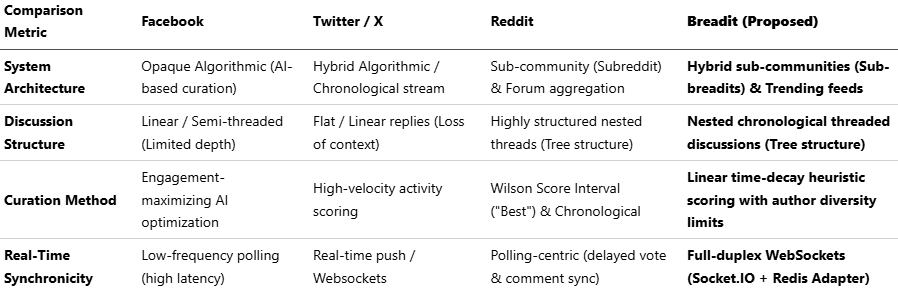
\includegraphics[width=0.92\linewidth,height=0.82\textheight,keepaspectratio]{images/image3.png}
\end{center}
